\documentclass[../Marcus.tex]{subfiles}

\begin{document}
	
\chapter{Number Fields and Number Rings}

\subsection*{Exercise 2.1}

(a) Given a number filed $K=\QQ(\alpha)$ with $[K:\QQ]=2$. Then $\alpha$ satisfies a polynomial in $\QQ[x]$ with degree 2. By clearing the denominators, we may assume that $\alpha$ satisfies $ax^2+bx+c$ where $a,b,c\in \ZZ$. So $\alpha=(-b\pm \sqrt{b^2-4ac})/(2a)$. This means $\QQ(\alpha)=\QQ(\sqrt{b^2-4ac})$.

(b) Given $\QQ(\sqrt{m}),\QQ(\sqrt{n})$ where $m,n$ are square-free and suppose $\QQ(\sqrt{m})=\QQ(\sqrt{n})$, we want to show $m=n$. We may assume none of $m,n$ is 1. (If one of them is 1, then the other will automatically be 1). Write $\sqrt{m}=a+b\sqrt{n}$, $a,b\in\QQ$, then $m=a^2+b^2n+2ab\sqrt{n}$. So $ab=0$.

If $a=0$, then $m=b^2n$. As $m$ is square-free, we must have $m=n$ (check this!). If $b=0$, then $m=a^2$. As $m$ is square-free, $m=1$ (check this!), which is not the case.

Now, suppose $\exists \phi:\QQ(\sqrt{m})\isoto\QQ(\sqrt{n})$. Since $\phi(1)=1$, we have $\phi |_\QQ=\id_\QQ$. Note that $m=\phi(m)=(\phi(\sqrt{m}))^2$. So $\phi(\sqrt{m})=\pm \sqrt{m}\in \QQ(\sqrt{n})$. This means $\QQ(\sqrt{m})\subseteq\QQ(\sqrt{n})$. Similarly, by using $\phi^{-1}$, we have $\QQ(\sqrt{n})\subseteq\QQ(\sqrt{m})$. So $\QQ(\sqrt{m})=\QQ(\sqrt{n})$, a contradiction.

\subsection*{Exercise 2.2}

$I=(2,1+\sqrt{-3})$. Since $(2)=2\ZZ\oplus2\ZZ\sqrt{-3}$. So $1+\sqrt{-3}\notin(2)$ and hence $I\neq(2)$. Moreover, $I^2=(4,2+2\sqrt{-3},-2+2\sqrt{-3})$ and $2I=(4,2+2\sqrt{-3})$. So it's sufficient to show $-2+2\sqrt{-3}\in 2I$. But this is easily seen because $-2+2\sqrt{-3}=-1(4)+1(2+2\sqrt{-3})$. So we have two different factorizations of ideals $J:=I^2=2I$.

Write $R=\ZZ[\sqrt{-3}]=\ZZ\oplus\ZZ\sqrt{-3}$. We first claim that $I$ is a prime ideal. Viewing $R$ and these ideals as additive groups. Since $\#(R/(2))=4$ and $(2)\subseteq I$, we have $\#(R/I)=1,2,4$. $1$ is impossible because if $I=R$ then $I^2=2I=R$ which is absurd. $4$ is also impossible because $(2)\varsubsetneq I$. Hence $\#(R/I)=2$ and so $R/I\simeq \ZZ/2\ZZ$, which is a field. This shows that $I$ is a maximal ideal and thus a prime ideal.

Now if $P\neq I$ is another prime ideal s.t. $(2)\subseteq P$. Then there exists $r\notin P$ and $r\in I$. (This is possible since we know $I$ is a maximal ideal so $I\varsubsetneq P$.) From $r\notin P$ we have $r^2\notin P$. On the other hand, from $r\in I$ we have $r^2\in I^2=2I \subseteq (2)\subseteq P$ so $r^2\in P$, which is absurd. This proves the uniqueness.

If $(2)=P_1\cdots P_n$ is a product of prime ideals, then for each $i$ we have $(2)\subseteq P_i$ and so $P_i=I$. This means $(2)=I^n$. Note that $n$ cannot be $1$, so we may write $(2)=I^2J=2IJ$ for some ideal $J$. (If $n=2$, $J=R$.) This is absurd because we know $(2)=2R\varsupsetneq 2I \supseteq 2IJ$.

\subsection*{Exercise 2.3}

If $\alpha=r+s\sqrt{m}$, then $\alpha$ satisfies $x^2-2rx+r^2-ms^2$. So $\alpha$ is an algebraic integer iff $2r,r^2-ms^2\in\ZZ$. First note that if $2r,r^2-ms^2\in\ZZ$, then so are $4r^2,4r^2-4ms^2$. Thus $4ms^2=m(2s)^2\in\ZZ$. As $m$ is square-free, we have $2s\in\ZZ$. Write $u=2r\in\ZZ$ and $v=2s\in\ZZ$. Since $4r^2-4ms^2=u^2-mv^2\in 4\ZZ$, we have $u^2 \equiv mv^2 \pmod{4}$.

case1: $m \equiv 2,3 \pmod{4}$. Then $u^2 \equiv 2v^2,3v^2 \pmod{4}$. This forces $v^2 \equiv 0 \pmod{4}$. So $v$ is even and $u^2 \equiv 0 \pmod{4}$, thus $u,v$ are both even. Hence, $r,s\in \ZZ$. This shows $\alpha=r+s\sqrt{m}\in \ZZ+\ZZ\sqrt{m}$. Conversely, showing $a+b\sqrt{m}$ where $a,b\in\ZZ$ is an algebraic integer is trivial.

case2: $m \equiv 1 \pmod{4}$. Observe that $\alpha=r+s\sqrt{m}=(2r+2s\sqrt{m})/2$. And from $u^2 \equiv v^2 \pmod{4}$, we have $u \equiv v \pmod{2}$, i.e., $2r \equiv 2s \pmod{2}$. Conversely, showing $(a+b\sqrt{m})/2$ where $a \equiv b \pmod{2}$ is an algebraic integer is straightforward. We skip the details.

\subsection*{Exercise 2.4}

Each $a_i$ is a root of a monic polynomial in $\ZZ[x]$. Let $e_i$ be the degree of such polynomial $f_i(x)$. We claim that $$G:=\{a_0^{m_0}a_1^{m_1}\cdots a_{n-1}^{m_{n-1}}\alpha^m \mid 1\leq m_i \leq e_i-1,1\leq m\leq n-1\}$$ is a set of generators of $\ZZ[a_0,\ldots,a_{n-1},\alpha]$. Indeed, given $a_0^{k_0}a_1^{k_1}\cdots a_{n-1}^{k_{n-1}}\alpha^k$. If $k_i\geq e_i$ for some $k_i$, then we may express $a_i^{k_i}$ as a linear combination of $1,a_i,a_i^2,\ldots,a_i^{e_i-1}$ over $\ZZ$ by exploiting $f_i(x)$. And if $k\geq n$, exploiting the equation $\alpha^n+a_{n-1}\alpha^{n-1}+\cdots+a_1\alpha+a_0$. In either case, we may reduce the exponents $k_0,\ldots,k_{n-1},k$ and express $a_0^{k_0}a_1^{k_1}\cdots a_{n-1}^{k_{n-1}}\alpha^k$ as a linear combination of the elements in $G$ over $\ZZ$.

Thus, $\ZZ[a_0,\ldots,a_{n-1},\alpha]$ has a finitely generated additive group. And by Thm 2(3) (p. 11), $\alpha$ is an algenraic integer.  

\subsection*{Exercise 2.5}

Induction on $n:=\#\{\text{terms of }f\}$. $n=1$, write $f(x)=ax^i \in \ZZ_p[x]$. Since $a^p \equiv a \pmod{p}$, we have $f(x^p)=ax^{pi}=a^px^{pi}=(ax^i)^p=f(x)^p$ in $\ZZ_p[x]$

Suppose when $n=k-1$, the statement holds. Consider $n=k$. Write $f(x)=a_1x^{i_1}+a_2x^{i_2}+\cdots+a_kx^{i_k}$. Let $g(x)$ be the sum of first $k-1$ terms. Then $f(x)=g(x)+a_kx^{i_k}$ and $$f(x^p)=g(x^p)+a_kx^{pi_k}=g(x)^p+(a_kx^{i_k})^p=\left(g(x)+a_kx^{i_k}\right)^p=f(x)^p$$

\subsection*{Exercise 2.6}

Write $g=f^2h$, then $g'=2ff'h+f^2h'$. Since $f\mid 2ff'h$ and $f\mid f^2h'$, we have $f\mid 2ff'h+f^2h'=g'$.

\subsection*{Exercise 2.7}

We've obtained a bijection $\phi: \Gal(\QQ(\omega)/\QQ)\to\ZZ_m^{\times}$ in the proof of Cor 2 (p. 13). Now, for $\sigma\in \Gal(\QQ(\omega)/\QQ)$, $\sigma(\omega)=\omega^k$, define $\phi(\sigma):=k\in\ZZ_m^{\times}$. We check that $\phi$ is a homomorphism. Given $\sigma,\tau\in\Gal(\QQ(\omega)/\QQ)$ and assume $\sigma(\omega)=\omega^k,\tau(\omega)=\omega^h$, then we have $\phi(\sigma)=k, \phi(\tau)=h$ and $(\sigma\circ\tau)(\omega)=\omega^{hk}$. Hence, $\phi(\sigma\circ\tau)=hk=\phi(\sigma)\phi(k)$.

\subsection*{Exercise 2.8}

(a) We know
$\disc(\omega)=\pm p^{p-2}$ where $+$ holds iff $p\equiv 1 \pmod{4}$. Since $\sigma(\omega^k)\in\QQ(\omega)$ for each embedding of $\QQ(\omega)$ in $\CC$ and each $k\in\NN$, we have $\sqrt{\disc(\omega)}=\sqrt{\pm p^{p-2}} \in \QQ(\omega)$. Also note that $\sqrt{p^{p-1}} \in \ZZ \subset \QQ(\omega)$. So if $p\equiv 1 \pmod{4}$, then $\sqrt{p^{p-1}}/\sqrt{p^{p-2}} = \sqrt{p} \in \QQ(\omega)$. And if $p\equiv 3 \pmod{4}$, then $\sqrt{p^{p-1}}/\sqrt{-p^{p-2}} = -i\sqrt{p} \in \QQ(\omega)$, so $\sqrt{-p}\in\QQ(\omega)$.

Consider $\sqrt{-3}$. In this case take $p=3$ and $\omega=e^{2\pi i/3}$. So $$\disc(\omega)=
\begin{vmatrix}
1 & \omega \\
1 & \omega^2
\end{vmatrix}^2
=(\omega^2-\omega)^2=-3$$
One may check that $\sqrt{-3}=-(\omega^2-\omega)=\omega-\omega^2$.
On the other hand, condiser $\sqrt{5}$. In this case take $p=5$ and $\omega=e^{2\pi i/5}$. So $$\disc(\omega)=
\begin{vmatrix}
1 & \omega & \omega^2 & \omega^3 \\
1 & \omega^2 & \omega^4 & \omega^6 \\
1 & \omega^3 & \omega^6 & \omega^9 \\
1 & \omega^4 & \omega^8 & \omega^{12} 
\end{vmatrix}^2=(-5\omega^4+5\omega^3+5\omega^2-5\omega)^2=5^3
$$
This gives us $(\omega^4-\omega^3-\omega^2+\omega)^2=5$. One may check that $\sqrt{5}=\omega^4-\omega^3-\omega^2+\omega$.

(b) $w=e^{2\pi i/8}=\cos\frac{\pi}{4}+i\sin\frac{\pi}{4}=\frac{\sqrt{2}}{2}+\frac{\sqrt{2}}{2}i$. So $\QQ(\omega)=\QQ(\sqrt{2}(1+i)/2)$. Since $\omega^2=i$, we have $i\in\QQ(\omega$). Hence, $\sqrt{2}\in\QQ(\omega)$. 

(c) Write $d:=\disc(\mathbb{A}\cap\QQ(\sqrt{m})$. We use $\QQ(\omega_k)$ to denote the $k$-th cyclotomic field for $k\in\NN$. Let $m=\sgn(m)2^ep_1p_2\cdots p_k$ be the prime factorization of $m$. If $p_i\equiv 3 \pmod{4}$, write $p_i=-(-p_i)$ where $-p_i\equiv 1 \pmod{4}$. So we may rewrite $m=(-1)^n2^ep_1p_2\cdots p_k$ where $p_i\equiv 1 \pmod{4}$ for all $i$.

Note that if $p_i>0$, then $p_i\equiv 1 \pmod{4}$ and by (a) we know $\sqrt{p_i}\in\QQ(\omega_{p_i})$. And if $p_i<0$, then $-p_i\equiv 3 \pmod{4}$ and by (a) again we know $\sqrt{-(-p_i)}=\sqrt{p_i} \in\QQ(\omega_{-p_i})$. So in either case we have $\sqrt{p_i}\in\QQ(\omega_{|p_i|})$.

We first assume $e=0$, i.e., $m$ is odd. If $n$ is even, then $m=p_1p_2\cdots p_k\equiv 1 \pmod{4}$. So $d=m$, and we have
$$\sqrt{m}=\sqrt{p_1p_2\cdots p_k}=\pm \sqrt{p_1}\cdots \sqrt{p_k}\in\QQ(\omega_{|m|})$$ where the $\pm$ depends on $\sgn(m)$ (consider $m=3\cdot7$ and $-5\cdot7$). And if $n$ is odd, then $m=-p_1p_2\cdots p_k\equiv 3 \pmod{4}$. So $d=4m$. Since $\QQ(\sqrt{-1})=\QQ(\omega_4)\subset\QQ(\omega_{|4m|})$, we have $$\sqrt{m}=\sqrt{-p_1p_2\cdots p_k}\in\QQ(\omega_{|4m|})$$

On the other hand, if $e=1$, then $m\equiv 2\pmod{4}$, so $d=4m$. By (b) we have $\sqrt{2}\in\QQ(\omega_8)\subset\QQ(\omega_{|4m|})$ and hence $\sqrt{m}\in\QQ(\omega_{|4m|})$.
 
\subsection*{Exercise 2.9}

Write $\theta=e^{2\pi ih/k}$ where $\gcd(h,k)=1$. Since $r=\lcm(k,m)$. We then write $r=kk'=mm'$ where $k',m'\in\ZZ$. We claim that $\gcd(m',k'h)=1$. First note that from the definition of $r$, we have $\gcd(k',m')=1$. Moreover, if there exists a prime $p$ s.t. $p\mid m'$ and $p\mid h$, then $p\mid mm'=r=kk'$. so $p\mid k$ or $p\mid k'$. Both cases are impossible from the fact that $\gcd(h,k)=\gcd(k',m')=1$. This means $\gcd(m',h)=1$ and hence the claim is done.

Now, take $u,v\in\ZZ$ s.t. $1=um'+vk'h$. Then $1/r=u/m+vh/k$ and thus $$e^{\frac{2\pi i}{r}}=e^{\frac{2\pi iu}{m}}e^{\frac{2\pi ivh}{k}}=\omega^u\theta^v$$

\subsection*{Exercise 2.10}

If $r\neq m$, then $r<m$. Write $m=2^{e_0}\prod_{i=1}^s p_i^{e_i}$, $r=2^{f_0}\prod_{j=1}^t p_j^{f_j}$. Then we have $e_0\geq 1,s\leq t$ and
$e_i\leq f_i$, $\forall i=0,1,\ldots,s$. Note that $$\phi(m)=2^{e_0-1}\prod_{i=1}^s (p_i-1)p_i^{e_i-1},\ \phi(r)=2^{f_0-1}\prod_{j=1}^s (p_j-1)p_j^{f_j-1}\prod_{j=s+1}^t (p_j-1)p_j^{f_j-1}$$

If $s<t$, i.e., $r$ has some prime divisor which does not divide $m$. Then $$\phi(r)\geq \phi(m)\prod_{j=s+1}^t (p_j-1)p_j^{f_j-1} > \phi(m)$$ which is a contradiction. This means $r,m$ have the same prime divisors, i.e., $r=2^{f_0}\prod_{i=1}^s p_i^{f_i}$.

Moreover, from $\phi(r)\leq \phi(m)$, we have $$2^{f_0-1}\prod_{i=1}^s (p_i-1)p_i^{f_i-1}\leq 2^{e_0-1}\prod_{i=1}^s (p_i-1)p_i^{e_i-1}$$ By canceling the terms we get $$2^{f_0-e_0}\prod_{i=1}^s p_i^{f_i-e_i}\leq 1$$ This inequality implies $f_i=e_i$ for all $i=0,1,\ldots,s$. Hence, $r=m$.
\subsection*{Exercise 2.11}

(a) We may write $$f(x)=(x-e^{i\theta_1})(x-e^{i\theta_2})\cdots(x-e^{i\theta_n})=x^n+c_1x^{n-1}+\cdots+c_{n-1}x+c_n$$ Observe that the coefficient of $x^r$ is $$c_{n-r}=\sum (-1)^{n-r}e^{i\theta_{k_1}}e^{i\theta_{k_2}}\cdots e^{i\theta_{k_{n-r}}}$$ where the sum is among all subsets $I=\{k_1,\ldots,k_{n-r}\} \subset \{1,\ldots,n\}$. Hence, $$|c_{n-r}|\leq \sum \left|(-1)^{n-r}e^{i\theta_{k_1}}e^{i\theta_{k_2}}\cdots e^{i\theta_{k_{n-r}}}\right| =\sum 1=\binom{n}{n-r}=\binom{n}{r}$$

(b) Fix $n$, let $\Fcal$ be the set of all irreducible polynomials of $\alpha\in\Ocal_K$ s.t. $\deg\Irr_{\QQ}(\alpha)=n$ and all roots of $\Irr_{\QQ}(\alpha)$ have absolute value 1. Since $\Fcal\subset\ZZ[x]_+$, by (a), we know $\Fcal$ is a finite set. Since every algebraic integer with the desired properties must be a root of some polynomial in $\Fcal$, the results follows.

(c) For each $k\in\NN$, we know $m:=[\QQ(\alpha^k):\QQ] \leq n$. There are $m$ embeddings of $\QQ(\alpha^k)$ in $\CC$. And the $m$ conjugates of $\alpha^k$ are $\{\sigma_i(\alpha^k)\mid i=1,\ldots,m\}$. Extend all $\sigma_i$ to some embedding of $\QQ(\alpha)$ in $\CC$, still denote it as $\sigma_i$. Let $\alpha_1,\ldots,\alpha_n$ be the $n$ conjugates of $\alpha$. Since $\sigma_i(\alpha^k)=\sigma_i(\alpha)^k=\alpha_j^k$ for some $j$, we know the $m$ conjugates of $\alpha^k$ are the set $\{\alpha_1^k,\ldots,\alpha_n^k\}$. Moreover, $|\sigma_i(\alpha^k)|=|\sigma_i(\alpha)^k|=1$.

Since all $\alpha^k$ has degree $\leq n$, consider $\{\alpha,\alpha^2,\alpha^3,\cdots\} \subset \cup_{i=1}^n \Acal_i$ where $\Acal_i$ is the set of algebraic integers with degree $i$ s.t. all of whose conjugates have absolute value 1. Since the RHS is a finite set by (b), so is the LHS. Hence, $\exists i< j$ s.t. $\alpha^i=\alpha^j$, i.e., $\alpha^{j-i}=1$.

\subsection*{Exercise 2.12}

(a) Note that the embeddings of $\QQ(\omega)$ in $\CC$ are in fact automorphisms in $\QQ(\omega)$ and the complex conjugation is one of the embedding because $\ovl{\omega}=\omega^{-1}=\omega^{p-1}$. Also recall that $\Gal(\QQ(\omega)/\QQ)$ is an abelian group. Thus, for each embedding $\sigma_i$, we have $$\left|\sigma\left(\frac{u}{\ovl{u}}\right)\right| = \left|\frac{\sigma(u)}{\sigma(\ovl{u})}\right| = \left|\frac{\sigma(u)}{\ovl{\sigma(u)}}\right| = 1$$ By Ex 2.11(c), we have $u/\ovl{u}$ is a root of unity. Moreover, by Cor 3 of Thm 3 (p. 14), $u/\ovl{u}\in\QQ(\omega)$ must be a $2p$-th root of unity, which are precisely $\pm \omega^k$, $k\in\ZZ$.

(b) If $u/\ovl{u}=-\omega^k$, then it's easy to see that $u^p=-\ovl{u^p}$. By Ex 1.25, $u^p\equiv a \pmod{p}$ for some integer $a$. Thus, $u^p \equiv a = \ovl{a} \equiv \ovl{u^p} = -u^p \equiv -a \pmod{p}$. So $2a\equiv 0 \pmod{p}$, and thus $a\equiv u^p \equiv0 \pmod{p}$, i.e., $p\mid u^p$. Since $u^p$ is a unit, so is $p$, a contradiction.

\subsection*{Exercise 2.13}

Recall that we have
$$
\Ocal_{\QQ\sqrt{m}}=
\begin{cases}
\{ a+b\sqrt{m}\mid a,b\in\ZZ \} & \text{if } m \equiv 2,3 \pmod{4}\\
\{ (a+b\sqrt{m})/2 \mid a,b\in\ZZ,a \equiv b \pmod{2} \} & \text{if } m \equiv 1 \pmod{4}
\end{cases}
$$
And also note that $r+s\sqrt{m}\in \Ocal_{\QQ\sqrt{m}}$ is a unit iff $\Nr(r+s\sqrt{m})=r^2-ms^2=\pm1$.

We first treat the case $m=-1,-3$. If $m=-1 \equiv 3 \pmod{4}$, the integral solutions of $a^2+b^2=\pm1$ are $(a,b)=(\pm1,0),(0,\pm1)$. So the units are $1,-1,i,-i$. And if $m=-3 \equiv 1 \pmod{4}$. $\Nr((a+b\sqrt{-3})/2)=a^2/4+3b^2/4=\pm1$ iff $a^2+3b^2=\pm4$. The integral solutions are $(a,b)=(\pm1,\pm1),(\pm2,0)$. So we have 6 units.

Now, assume $m\neq-1,-3$. If $m \equiv 2,3 \pmod{4}$, then the integral solutions of $a^2-mb^2=\pm1$ are $(a,b)=(\pm1,0)$. So the units are $1,-1$. If $m \equiv 1 \pmod{4}$. $\Nr((a+b\sqrt{m})/2)=a^2/4-mb^2/4=\pm1$ iff $a^2-mb^2=\pm4$. The integral solutions are precisely $(a,b)=(\pm2,0)$ So the units are $1,-1$.

\subsection*{Exercise 2.14}

$1/(1+\sqrt{2})=-1+\sqrt{2}\in \ZZ[\sqrt{2}]$. So $1+\sqrt{2}$ is a unit. Moreover, for each $k\in\NN$, $(1+\sqrt{2})^k>\sqrt{2}^k>1$. So $1+\sqrt{2}$ can't be a root of $1$.

Write $(1+\sqrt{2})^k=a_k+b_k\sqrt{2}$. Since $\Nr(1+\sqrt{2})=-1$, we have $$\Nr(a_k+b_k\sqrt{2})=\Nr((1+\sqrt{2})^k)=\left(\Nr(1+\sqrt{2})\right)^k=(-1)^k.$$ Hence, $a_k+b_k\sqrt{2}$ are all units.

\subsection*{Exercise 2.15}

(a) $\Nr(a+b\sqrt{-5})=a^2-5b^2$. Suppose $a^2-5b^2=2,3$ has integral solution. Then $a^2-5b^2 \equiv a^2-b^2 \equiv 2 \pmod{4}$, which is impossible. And $a^2-5b^2 \equiv a^2 \equiv 3 \pmod{5}$, which is also impossible.

(b) $2\cdot3=(1+\sqrt{-5})(1-\sqrt{-5})=6$. Since by Ex 2.13, $\pm1$ are the only units in $\ZZ[\sqrt{-5}]$. So $2,3,1+\sqrt{-5},1-\sqrt{-5}$ are pairwise nonaassociated. Hence, the above factorizations are distinct.

\subsection*{Exercise 2.16}

If $\sqrt{3}\in\QQ(\alpha)$, write $\sqrt{3}=a+b\alpha+c\alpha^2+d\alpha^3$. It's easy to see that the four conjugates of $\alpha$ are $\pm\alpha,\pm\alpha i$ and $\Tr(\alpha)=\Tr(\alpha^2)=\Tr(\alpha^3)=0$. On the other hand, since $\QQ(\sqrt{3})\subset\QQ(\alpha)$, the two embeddings of $\QQ(\sqrt{3})$ in $\CC$ can be extended to the four embeddings of $\QQ(\alpha)$ in $\CC$. Two of them map $\sqrt{3}$ to $\sqrt{3}$ and the other two map $\sqrt{3}$ to $-\sqrt{3}$. So $\Tr(\sqrt{3})=0$ and hence we have $$0=\Tr(\sqrt{3})=\Tr(a+b\alpha+c\alpha^2+d\alpha^3)=4a, \ a=0$$

From $\sqrt{3}=b\alpha+c\alpha^2+d\alpha^3$ we have $\sqrt{3}/\alpha=b+c\alpha+d\alpha^2$. Let $\beta:=\sqrt{3}/\alpha=\sqrt[4]{9/2}$. The four conjugates of $\beta$ are $\pm\beta,\pm\beta i$ and so $\Tr(\beta)=0$. Hence, we have $$0=\Tr(\beta)=\Tr(b\alpha+c\alpha^2+d\alpha^3)=4b, \ b=0$$

From  $\sqrt{3}=c\alpha^2+d\alpha^3$ we have $\sqrt{3}/\alpha^2=c+d\alpha$. Similar to the argument of $\Tr(\sqrt{3})=0$, we know $\Tr(\sqrt{3}/\alpha^2)=0$. Thus we have $c=0$. And from $\sqrt{3}=d\alpha^3$ we have $d=\sqrt{3}/\alpha^3$. This is a contradiction because $d\in\QQ$.

\subsection*{Exercise 2.17}

$\alpha\in L$. Consider the field extensions $K\subset K(\alpha)\subset L$ where $[L:K]=n$ and $[K(\alpha):K]=d$. We first compute $\tr(\alpha)$ and $\nr(\alpha)$. Since $\Irr_\QQ(\alpha)$ has degree $d$, take $c_1,\ldots,c_d\in\QQ$ s.t. $\alpha^d+c_1\alpha^{d-1}+\cdots+c_d=0$. Hence, $\tr(\alpha)=-c_1$ and $\nr(\alpha)=(-1)^{d}c_d$.

Next, let $\{\beta_1,\ldots,\beta_{n/d}\}$ be a basis of $L$ over $K(\alpha)$. For each $x\in L$, we may write
\begin{align*}
x &= x_1\beta_1+\cdots+x_{n/d}\beta_{n/d} \\ &=(x^{(1)}_{1}+x^{(2)}_{1}\alpha+\cdots+x^{(d)}_{1}\alpha^{d-1})\beta_1+\cdots+(x^{(1)}_{n/d}+x^{(2)}_{n/d}\alpha+\cdots+x^{(d)}_{n/d}\alpha^{d-1})\beta_{n/d}
\end{align*} in a unique way. Thus $\{\alpha^{i}\beta_j\mid 0\leq i\leq d-1,1\leq j \leq n/d\}$ is a basis of $L$ over $K$. By basic linear algebra we know that $$A=\begin{bmatrix}
A_1 &         &             &               \\
       & A_2 &             &               \\
       &         & \ddots &               \\
       &         &             & A_{n/d}
\end{bmatrix}, \text{where }
A_i=\begin{bmatrix}
0          & 0  & \cdots & 0         & -c_d       \\
1           & 0 & \cdots & 0          & -c_{d-1} \\
0          & 1  & \cdots & 0          & -c_{d-2}     \\
\vdots &     & \ddots & \vdots & \vdots       \\
0         & 0  & \cdots & 1           & -c_1       \\
\end{bmatrix}
$$
It's easy to see that $\tr(A_i)=-c_1=\tr(\alpha)$ and $\det(A_i)=(-1)^dc_d=\nr(\alpha)$ for all $i$. Hence by Thm 4$'$ (p. 17),
\begin{align*}
\tr(A)&=\frac{n}{d}\tr(A_i)=\frac{n}{d}\cdot\tr(\alpha)=\Tr^L_K(\alpha)\\
\det(A)&=\det(A_i)^{n/d}=(\nr(\alpha))^{n/d}=\Nr^L_K(\alpha)
\end{align*}

\subsection*{Exercise 2.18}

Let $\sigma_{i_1}\tau_{j_1},\sigma_{i_2}\tau_{j_2}$ be two automorphisms of $N$ which agree on $M$. Thus they agree on $L$, i.e., $\sigma_{i_1}(\tau_{j_1}(x))=\sigma_{i_2}(\tau_{j_2}(x))$ $\forall x\in L$. Since $\tau_{j_1},\tau_{j_2}$ fix $L$ pointwise, we have $\sigma_{i_1}(x)=\sigma_{i_2}(x)$ $\forall x\in L$. So $\sigma_{i_1},\sigma_{i_2}$ agree on $L$. This means $i_1=i_2$. We then write $\sigma:=\sigma_{i_1}=\sigma_{i_2}$.

From the assumption $\sigma\tau_{j_1},\sigma\tau_{j_2}$ agree on $M$, we apply $\sigma^{-1}$ and get $\tau_{j_1},\tau_{j_2}$ agree on $M$. This means $j_1=j_2$. Conclude that $\sigma_{i_1}\tau_{j_1}=\sigma_{i_2}\tau_{j_2}$.

\subsection*{Exercise 2.19}

Induction on $n$. Suppose the result holds for $n$, i.e.,
$$
\det\begin{pmatrix}
1           & a_1      & \cdots & a_1^{n-1} \\
1           & a_2     & \cdots & a_2^{n-1} \\
\vdots & \vdots & \ddots & \vdots \\
1          & a_n      & \cdots & a_n^{n-1}
\end{pmatrix}=\prod_{1\leq r<s\leq n}(a_s-a_r)
$$
Consider $n+1$. We first claim that for any monic polynomial $f\in R[x]$ of degree $n$, we have
$$
\det\begin{pmatrix}
1           & a_1       & \cdots & a_1^{n-1}         & a_1^n \\
1           & a_2       & \cdots & a_2^{n-1}        & a_2^n \\
\vdots & \vdots   & \ddots & \vdots              & \vdots \\
1          & a_n        & \cdots & a_n^{n-1}        & a_n^n \\
1          & a_{n+1} & \cdots & a_{n+1}^{n-1} & a_{n+1}^n
\end{pmatrix}=
\det\begin{pmatrix}
1           & a_1        & \cdots & a_1^{n-1}       & f(a_1)\\
1           & a_2       & \cdots & a_2^{n-1}       & f(a_2) \\
\vdots & \vdots   & \ddots & \vdots              & \vdots \\
1          & a_n        & \cdots & a_n^{n-1}        & f(a_n) \\
1          & a_{n+1} & \cdots & a_{n+1}^{n-1} & f(a_{n+1})
\end{pmatrix}
$$
Given $f(x)=x^n+c_{n-1}x^{n-1}+\cdots+c_0$. Observe that the RHS is
$$
\det\begin{pmatrix}
1          & a_1         & \cdots & a_1^{n-1}        & a_1^n+c_{n-1}a_1^{n-1}+\cdots+c_0\\
1          & a_2        & \cdots & a_2^{n-1}        & a_2^n+c_{n-1}a_2^{n-1}+\cdots+c_0 \\
\vdots & \vdots   & \ddots & \vdots              & \vdots \\
1          & a_n        & \cdots & a_n^{n-1}        & a_n^n+c_{n-1}a_n^{n-1}+\cdots+c_0 \\
1          & a_{n+1} & \cdots & a_{n+1}^{n-1} & a_{n+1}^n+c_{n-1}a_{n+1}^{n-1}+\cdots+c_0
\end{pmatrix}$$
Let $\Ccal_1,\ldots,\Ccal_{n+1}$ be the column vetcors of the matrix corresponding to the above determinant. If $c_i\neq 0$, by using the column operation $-c_i\cdot\Ccal_{i+1}+\Ccal_{n+1}$, we get the matrix correspond to the LHS. Since these operations leave the determinant unchanged, the claim is done.

In particular, take $f(x)=(x-a_1)(x-a_2)\cdots(x-a_n)$. Then we have
$$
\begin{aligned}
\lhs &= \det\begin{pmatrix}
1           & a_1        & \cdots & a_1^{n-1}        & 0 \\
1           & a_2        & \cdots & a_2^{n-1}       & 0 \\
\vdots & \vdots    & \ddots & \vdots              & \vdots \\
1           & a_n        & \cdots & a_n^{n-1}        & 0 \\
1           & a_{n+1} & \cdots & a_{n+1}^{n-1} & f(a_{n+1})
\end{pmatrix}
=
f(a_{n+1})
\det\begin{pmatrix}
1           & a_1      & \cdots & a_1^{n-1} \\
1           & a_2     & \cdots & a_2^{n-1} \\
\vdots & \vdots & \ddots & \vdots \\
1          & a_n      & \cdots & a_n^{n-1}
\end{pmatrix} \\
&= f(a_{n+1})\prod_{1\leq r<s\leq n}(a_s-a_r) \\
&= (a_{n+1}-a_1)(a_{n+1}-a_2)\cdots(a_{n+1}-a_n)\prod_{1\leq r<s\leq n}(a_s-a_r)  \\
&= \prod_{1\leq r<s\leq n+1}(a_s-a_r)
\end{aligned}
$$

\subsection*{Exercise 2.20}

Write $f(x)=(x-\alpha)g(x)$ where $g(x)=(x-\beta_2)\cdots(x-\beta_n)$. By differentiating we get $f'(x)=g(x)+(x-\alpha)g'(x)$. So $f'(\alpha)=g(\alpha)=(\alpha-\beta_2)\cdots(\alpha-\beta_n)$. Note that $f(x)$ has no repeated root because $K/\QQ$ is separable.

\subsection*{Exercise 2.21}

Let $K=\QQ(\alpha)$ where $\alpha\in\Ocal_K$ and $h(x):=\Irr_\QQ(\alpha)$. Given $f(x)\in\ZZ[x]_+$ s.t. $f(\alpha)=0$, then $h(x)\mid f(x)$. Write $f(x)=h(x)g(x)$, then by the Lem of Thm 1 (p. 10), $g(x)\in\ZZ[x]$. So $g(\alpha)\in\Ocal_K$.

We know $\disc(\alpha)=\pm \Nr(h'(\alpha))$, so it's enough to show $\Nr(h'(\alpha))\mid\Nr(f'(\alpha))$. From $f=hg$ we have $f'(\alpha)=h'(\alpha)g(\alpha)$. So $\Nr(f'(\alpha))=\Nr(h'(\alpha))\Nr(g(\alpha))$. Note that all three norms are integers so the results follows. (We've used the observation that $g(\alpha)\in\Ocal_K$.)

\subsection*{Exercise 2.22}

Extend all $\sigma_i$ to some normal extension $L$ of $\QQ$ so that they become automorphisms of $L$, still denote them as $\sigma_1,\ldots,\sigma_n$. Note that $\sigma_i(\alpha_j)\in \Ocal_L$. Moreover, observe that $P+N,PN$ remain unchanged by the actoin of each $\QQ$-automorphism of $L$. So by Galois theory we have $P+N,PN\in\QQ$. Hence, $P+N,PN\in\ZZ$. Hence, $d=(P+N)^2-4PN \equiv 0,1 \pmod{4}$.

\subsection*{Exercise 2.23 \color{red}(incomplete, missing (a))}

(b) Following the suggestion, we have three $(mn)\times(mn)$ matrices $A,B,AB$ where
$$A=\begin{bmatrix}
A_1 &         &             &               \\
       & A_2 &             &               \\
       &         & \ddots &               \\
       &         &             & A_{n}
\end{bmatrix}, \text{where }
A_i=\begin{bmatrix}
\sigma_i\tau_1(\beta_1) & \sigma_i\tau_1(\beta_2) & \cdots & \sigma_i\tau_1(\beta_m)  \\
\sigma_i\tau_2(\beta_1) & \sigma_i\tau_2(\beta_2) & \cdots & \sigma_i\tau_2(\beta_m) \\
\vdots &     & \ddots & \vdots       \\
\sigma_i\tau_m(\beta_1) & \sigma_i\tau_m(\beta_2) & \cdots & \sigma_i\tau_m(\beta_m) \\
\end{bmatrix}
$$
$$B=\begin{bmatrix}
\sigma_1(\alpha_1)\cdot I_m & \sigma_1(\alpha_2)\cdot I_m & \cdots & \sigma_1(\alpha_n)\cdot I_m  \\
\sigma_2(\alpha_1)\cdot I_m & \sigma_2(\alpha_2)\cdot I_m & \cdots & \sigma_2(\alpha_n)\cdot I_m  \\
\vdots & \vdots & \ddots & \vdots \\
\sigma_n(\alpha_1)\cdot I_m & \sigma_n(\alpha_2)\cdot I_m & \cdots & \sigma_n(\alpha_n)\cdot I_m
\end{bmatrix}
$$
$$AB=\begin{bmatrix}
A_1\sigma_1(\alpha_1) & A_1\sigma_1(\alpha_2) & \cdots & A_1\sigma_1(\alpha_n)  \\
A_2\sigma_2(\alpha_1) & A_2\sigma_2(\alpha_2) & \cdots & A_2\sigma_2(\alpha_n)  \\
\vdots & \vdots & \ddots & \vdots  \\
A_n\sigma_n(\alpha_1) & A_n\sigma_n(\alpha_2) & \cdots & A_n\sigma_n(\alpha_n)  \\
\end{bmatrix}
$$
Computing three determinants $|AB|,|A|,|B|$ carefully and one should be able to obtain the desired formula from the equation $|AB|^2=|B|^2|A|^2$. (No special tricks!)

(c) Consider the following diagram of field extensions
\begin{center}
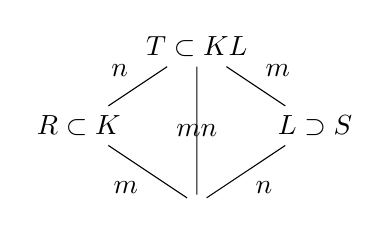
\begin{tikzpicture}
\draw (0,0) node (Q) {$\QQ$};
\draw (-1.5,1) node (K) {$R\subset K$};
\draw (1.5,1) node (L) {$L\supset S$};
\draw (0,2) node (E) {$T\subset KL$};
\draw (Q) -- node[below left] {$m$} (K) -- node[above left] {$n$} (E) -- node {$mn$} (Q) -- node[below right] {$n$} (L) -- node[above right] {$m$} (E);
\end{tikzpicture}
\end{center}
And by assumption we have $T=RS$. Let $\{\alpha_1,\ldots,\alpha_m\},\{\beta_1,\ldots,\beta_n\}$ be integral bases of $R,S$, respectively. Then $\{\alpha_i\beta_j\mid 1\leq i\leq m, 1\leq j\leq n\}$ is an integral basis of $T$ over $\QQ$. It's easy to check $\{\beta_1,\ldots,\beta_n\}$ forms an integral basis of $KL$ over $K$. By considering the tower of field extensions $\QQ\subset K\subset KL$ and using (b), we have
\begin{align*}
\disc^{KL}_\QQ(T) &= \disc^{KL}_\QQ(\alpha_1\beta_1,\ldots,\alpha_m\beta_n)\\
&= \left(\disc^K_\QQ(\alpha_1,\ldots,\alpha_m)\right)^n\cdot \Nr^K_\QQ\left(\disc^{KL}_K(\beta_1,\ldots,\beta_n)\right)\\
&= \disc(R)^n\cdot \Nr^K_\QQ\left(\disc(S)\right)\\
&= \disc(R)^n\disc(S)^m
\end{align*}

\subsection*{Exercise 2.24}

\subsection*{Exercise 2.25}

Since $\alpha$ is algebraic over $\QQ$, $\exists m_i,n_i \in \ZZ, m_i \neq 0, i=1,\ldots,k$ s.t. $$\alpha^k + \frac{n_1}{m_1}\alpha^{k-1} + \cdots + \frac{n_k}{m_k} = 0$$ 
Let $m:=m_1\cdots m_k\in\ZZ$. By doing some algebra, we have
\begin{align*}
0 &= m^k\alpha^k + n_1\frac{m}{m_1}m^{k-1}\alpha^{k-1} + \cdots + n_k\frac{m}{m_k}m^{k-1} \\
&= (m\alpha)^k + n_1\frac{m}{m_1}(m\alpha)^{k-1} + \cdots + n_k\frac{m}{m_k}m^{k-1}
\end{align*}
Note that $m/m_i \in \ZZ$, $\forall i=1,\ldots,k$. Hence, $m\alpha$ is an algebraic integer.

Next, given a finite set $\{\alpha_1,\ldots,\alpha_r\}$ of algebraic numbers. For each $\alpha_i$, choose $m_i\in \ZZ$ s.t. $m_i\alpha_i$ is an algebraic integer. Let $m:=m_1\cdots m_r$, then $\{m\alpha_1,\ldots,m\alpha_r\} \subset \Ocal_K$.

\subsection*{Exercise 2.26}

By taking the product of two integers corresponding to each $\beta_i,\gamma_i$ in Ex 2.25 there exists $m\in\ZZ$ s.t. $\{m\beta_1,\ldots,m\beta_n\},\{m\gamma_1,\ldots,m\gamma_n\}\subset\Ocal_K$. Since these two sets still generate the same additive subgroup of $K$, we may express each $m\beta_i$ to the linear combination of $\{m\gamma_1,\ldots,m\gamma_n\}$ over $\ZZ$. And by applying the $n$ embeddings of $K$ in $\CC$ to these $n$ equations we obtain
$$\begin{pmatrix}
m\sigma_1(\beta_1)  &  \cdots & m\sigma_1(\beta_n)  \\
m\sigma_2(\beta_1) &  \cdots & m\sigma_2(\beta_n)  \\
\vdots                         &  \ddots & \vdots  \\
m\sigma_n(\beta_1) &  \cdots & m\sigma_n(\beta_n)
\end{pmatrix}=
\begin{pmatrix}
m\sigma_1(\gamma_1)  &  \cdots & m\sigma_1(\gamma_n)  \\
m\sigma_2(\gamma_1) &  \cdots & m\sigma_2(\gamma_n)  \\
\vdots                         &  \ddots & \vdots  \\
m\sigma_n(\gamma_1) &  \cdots & m\sigma_n(\gamma_n)
\end{pmatrix}
\begin{pmatrix}
c_{11}  & c_{21} & \cdots & c_{n1} \\
c_{12} & c_{22} & \cdots & c_{n2} \\
\vdots & \vdots  & \ddots & \vdots \\
c_{1n} & c_{2n} & \cdots & c_{nn} \\
\end{pmatrix}
$$
Taking determinants and squaring we have $\disc(m\beta_1,\ldots,m\beta_n)=\disc(m\gamma_1,\ldots,m\gamma_n)\cdot C$. Note that these three are all integers by our adjustment. Hence, we have $\disc(m\gamma_1,\ldots,m\gamma_n)$ divides $\disc(m\beta_1,\ldots,m\beta_n)$. Using similar argument can show $\disc(m\beta_1,\ldots,m\beta_n)$ divides $\disc(m\gamma_1,\ldots,m\gamma_n)$ and so they are in fact the same. Hence, we have $$m^{2n}\disc(\beta_1,\ldots,\beta_n)=\disc(m\beta_1,\ldots,m\beta_n)=\disc(m\gamma_1,\ldots,m\gamma_n)=m^{2n}\disc(\gamma_1,\ldots,\gamma_n)$$ So the result follows.

\subsection*{Exercise 2.27 \color{red}(incomplete, missing (a) and (b))}

(d) Let $\beta_1,\ldots,\beta_n$ be an integral basis and by wrting each $\alpha_i$ to the linear combination of $\beta_1,\ldots,\beta_n$ over $\ZZ$ we obtain
$$\begin{pmatrix}
\alpha_1  \\
\alpha_2 \\
\vdots \\
\alpha_n
\end{pmatrix}=
\begin{pmatrix}
c_{11}  & c_{21} & \cdots & c_{1n} \\
c_{21} & c_{22} & \cdots & c_{2n} \\
\vdots & \vdots  & \ddots & \vdots \\
c_{n1} & c_{n2} & \cdots & c_{nn} \\
\end{pmatrix}
\begin{pmatrix}
\beta_1 \\
\beta_2 \\
\vdots \\
\beta_n
\end{pmatrix}$$
By applying the $n$ embeddings of $K$ in $\CC$ to these $n$ equations, taking determinants and squaring, we have $\disc(\alpha_1,\ldots,\alpha_n)=\disc(\beta_1,\ldots,\beta_n)\cdot \det(C^T)^2=\disc(R)\cdot \det(C)^2$ where $C\in\Mat_n(\ZZ)$ is the coefficients matrix above. If $\disc(\alpha_1,\ldots,\alpha_n)=\disc(R)$, then we have $\det(C)=\pm 1$. (Here we've used the fact that the discriminant of any integral basis is nonzero.) This means $C$ is invertible and $C^{-1}\in\Mat_n(\ZZ)$. By appying $C^{-1}$ to the system of equations above we may express each $\beta_i$ to the linear combination of $\alpha_1,\ldots,\alpha_n$ over $\ZZ$ (in a unique way, of course). This shows $\{\alpha_1,\ldots,\alpha_n\}$ is an integral basis.

(e) Using the same notation in (d) we have $\disc(\alpha_1,\ldots,\alpha_n)=\disc(R)\cdot \det(C)^2$ where $C\in\Mat_n(\ZZ)$. All three of them are integers, so if $\disc(\alpha_1,\ldots,\alpha_n)$ is sqaure-free then we must have $\det(C)^2=1$. Thus $\disc(\alpha_1,\ldots,\alpha_n)=\disc(R)$ and by (d) we have $\{\alpha_1,\ldots,\alpha_n\}$ is an integral basis.

\subsection*{Exercise 2.28}

(a) $f'(\alpha)=3\alpha^2+a$. From $\alpha^3+a\alpha+b=0$ we have $\alpha^2=-a-b/\alpha$. So $f'(\alpha)=3(-a-b/\alpha)+a=-(2a\alpha+3b)/\alpha$. (Note that since $f$ is irreducible, so $b\neq 0$. This means $\alpha$ as a root of $f$ can not be zero.)

(b) Checking $2a\alpha+3b$ is a root is straightforward. Let $g(x)$ be the polynomial as in (b), then $g(x)=f((x-3b)/2a)$. As $f$ is irreducible, so is $g$. So $$\Irr_\QQ(2a\alpha+3b)=g(x)\cdot (2a)^3=(x-3b)^3+a(2a)^2(x-3b)+b$$ Since $-\Nr(2a\alpha+3b)$ is the constant term of its irreducible polynomial, we have $$\Nr(2a\alpha+3b)=4a^3b+27b^3$$

(c) By Thm 8 (p. 19) and (a), we have $$\disc(\alpha)=-\Nr\left(\frac{-(2a\alpha+3b)}{\alpha}\right)=-(-1)^3\cdot\Nr(2a\alpha+3b)\cdot\Nr\left(\frac{1}{\alpha}\right)$$ Since $\Irr_\QQ(\alpha)=x^3+ax+b$, we have $\Nr(1/\alpha)=1/\Nr(\alpha)=1/(-b)$. Thus by (b), $$\disc(\alpha)=(4a^3b+27b^3)\cdot\frac{-1}{b}=-(4a^3+27b^2)$$

(d) First, the condition $\alpha$ satisfies $x^3-x-1$, which is irreducible, tells us $a=-1,b=-1$. So by (c) $\disc(\alpha)=-23$, which is square-free. By Ex 2.27(e), we have $\{1,\alpha,\alpha^2\}$ forms a integral basis.

Next, $\alpha$ satisfies $x^3+x-1$, which is also irreducible, tells us $a=1,b=-1$. So $\disc(\alpha)=-31$, which is also square-free. Thus we have the same conclusion.

\subsection*{Exercise 2.29}

(a) Let $R=\Ocal_{\QQ\sqrt{m}},S=\Ocal_{\QQ\sqrt{n}},T=\Ocal_K$. Then we have $\disc(R)=m$, $\disc(S)=n$ and $d=\gcd(\disc(R),\disc(S))=1$. So the conditions of Cor 1 of Thm 12 (p. 24) are satisfied. Hence, $$T=RS=\left(\ZZ\oplus\ZZ\frac{1+\sqrt{m}}{2}\right)\left(\ZZ\oplus\ZZ\frac{1+\sqrt{n}}{2}\right)$$ So $\{1,(1+\sqrt{m})/2,(1+\sqrt{n})/2,(1+\sqrt{m}+\sqrt{n}+\sqrt{mn})/4\}$ is an integral basis of $T$. Moreover, by Ex 2.23(c), $\disc(T)=\disc(R)^2\disc(S)^2=(mn)^2$.  

(b) Using the same notation as above, we have $\disc(R)=m,\disc(S)=4n$ and $d=\gcd(m,4n)=~1$. (Here we've used the fact that $m$ is odd.) So we can use the same theorem again. Hence, $$T=RS=\left(\ZZ\oplus\ZZ\frac{1+\sqrt{m}}{2}\right)\left(\ZZ\oplus\ZZ\sqrt{n}\right)$$ So $\{1,\sqrt{n},(1+\sqrt{m})/2,(\sqrt{n}+\sqrt{mn})/2\}$ is an integral basis of $T$. And by Ex 2.23(c) again, we have $\disc(T)=m^2(4n)^2=16(mn)^2$.

\subsection*{Exercise 2.30}

(a) Note that it's equivalent to show $g(\alpha)\in3\cdot\ZZ[\alpha]$ iff $\ovl{g}\in\ovl{f}\cdot(\ZZ/3\ZZ)[x]$. Consider two canonical ring homomorphisms $\ZZ[x]\to\ZZ[\alpha]/(3)$ and $\ZZ[x]\to(\ZZ/3\ZZ)[x]/(\ovl{f})$. They are clear surjective. Moreover, their kernals are both $(3,f(x))\subset\ZZ[x]$. So we have the isomorphisms. $$\ZZ[\alpha]/(3) \simeq \ZZ[x]/(3,f(x)) \simeq (\ZZ/3\ZZ)[x]/(\ovl{f})$$ So $g(\alpha)\in(3)$ iff $g(\alpha)=0$ in $\ZZ[\alpha]/(3)$ iff $\ovl{g}=0$ in $(\ZZ/3\ZZ)[x]/(\ovl{f})$ iff $\ovl{g}\in(\ovl{f})$.

(b) Suppose $\mathbb{A}\cap K=\ZZ[\alpha]$. First note that any combination of $\alpha_i\alpha_j,i\neq j$ has either a factor $-6$ or $-9$. So $3\mid\alpha_i\alpha_j$ in $\ZZ[\alpha]$ if $i\neq j$.

The four embeddings of $K$ into $\CC$ send $\sqrt{7}$ to $\pm\sqrt{7}$ and $\sqrt{10}$ to $\pm\sqrt{10}$. So it's not hard to see that $\Tr(\alpha_i^n)=\sum_{i=1}^4 \alpha_i^n$. On the other hand, observe that in the expanded form of $(\alpha_1+\alpha_2+\alpha_3+\alpha_4)^n$, all the terms are divisible by $3$ in $\ZZ[\alpha]$ by the previous argument, except for $\sum_{i=1}^4 \alpha_i^n$. So we have $\Tr(\alpha_i^n)=\sum_{i=1}^4 \alpha_i^n \equiv (\alpha_1+\alpha_2+\alpha_3+\alpha_4)^n =4^n \pmod{3}$ in $\ZZ[\alpha]$.

This implies $\Tr(\alpha_i^n)-4^n=3r$ for some $r\in\ZZ[\alpha]$. Note that since $\alpha_i$ is an algebraic integer, $\Tr(\alpha_i^n)\in\ZZ$. So $r\in\ZZ[\alpha]\cap\QQ=\mathbb{A}\cap K\cap\QQ=\ZZ$. Thus $\Tr(\alpha_i^n)\equiv4^n \equiv 1\pmod{3}$ in $\ZZ$. This means $\Tr(\alpha_i^n/3)=\Tr(\alpha_i^n)/3\notin\ZZ$. So $\alpha_i^n/3$ is not an algebraic integer and so $3\nmid \alpha_i^n$ in $\ZZ[\alpha]$.

(c) Since $\alpha_i\in\mathbb{A}\cap K=\ZZ[\alpha]$. Write $\alpha_i=f_i(\alpha)$ where $f_i\in\ZZ[x]$. For $i\neq j$, by (b) we know $3\mid \alpha_i\alpha_j=f_i(\alpha)f_j(\alpha)=f_if_j(\alpha)$ in $\ZZ[\alpha]$. So by (a) we have $\ovl{f}\mid\ovl{f_i}\cdot\ovl{f_j}$. On the other hand, $3\nmid \alpha_i^n=(f_i(\alpha))^n=f_i^n(\alpha)$ in $\ZZ[\alpha]$. So $\ovl{f}\nmid\ovl{f_i}^n$.

We know $(\ZZ/3\ZZ)[x]$ is a UFD. For each $i$, since $\ovl{f}\nmid\ovl{f_i}$, $\ovl{f}$ has an irreducible factor $\ovl{g_i}$ s.t. $\ovl{g_i}\nmid\ovl{f_i}$. Moreover, for $j\neq i$, $\ovl{g_i}\mid\ovl{f}\mid\ovl{f_i}\cdot\ovl{f_j}$. And since $\ovl{g_i}\nmid\ovl{f_i}$, we have $\ovl{g_i}\mid\ovl{f_j}$.

(d) For each $i=1,2,3,4$. Take such $\ovl{g_i}\in(\ZZ/3\ZZ)[x]$ as in (c) where $\ovl{g_i}\mid\ovl{f}$, $\ovl{g_i}\nmid\ovl{f_i}$ and $\ovl{g_i}\mid\ovl{f_j}$ for $j\neq i$. Since $f$ has degree at most 4, so is $\ovl{f}$. Thus $\deg\ovl{g_i}=1$ for all $i$.

The polynomials with degree one in $(\ZZ/3\ZZ)[x]$ are $x,x+1,x+2,2x,2x+1,2x+2$. But up to unit there're only three because $x\sim2x,x+1\sim2x+2,x+2\sim2x+1$. Since there're four $\ovl{g_i}$'s, $\exists i\neq j$ s.t. $\ovl{g_i}\sim \ovl{g_j}$. So $\ovl{g_j}\mid\ovl{g_i}\mid\ovl{f_j}$, a contradiction. 

\subsection*{Exercise 2.31}

Let $x=(\sqrt{3}+\sqrt{7})/2$, then it's easy to check that $x$ satisfies $x^4-5x^2+1$. So $x$ is an algebraic integer. Consider the following diagram of field extensions
\begin{center}
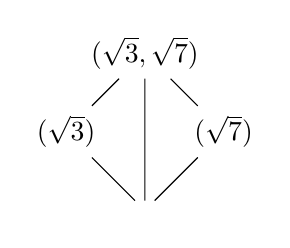
\begin{tikzpicture}
\draw (0,0) node (Q) {$\QQ$};
\draw (-1,1) node (K) {$\QQ(\sqrt{3})$};
\draw (1,1) node (L) {$\QQ(\sqrt{7})$};
\draw (0,2) node (E) {$\QQ(\sqrt{3},\sqrt{7})$};
\draw (Q) -- (K) -- (E) -- (Q) -- (L) -- (E);
\end{tikzpicture}
\end{center}
Let $R=\ZZ[\sqrt{3}],S=\ZZ[\sqrt{7}],T$ be the rings of algebraic integers of $\QQ(\sqrt{3}),\QQ(\sqrt{7}),\QQ(\sqrt{3},\sqrt{7})$, respectively. Then we have $x\in T$, and it's easy to see that $x\notin RS$. Thus, $RS\varsubsetneq T$. 

Note that we have $\disc(R)=12$ and $\disc(S)$=28, so $d:=\gcd(\disc(R),\disc(S))=4\neq1$.

\subsection*{Exercise 2.32}

\subsection*{Exercise 2.33}

$\Nr(\omega)=\prod_{k} \omega^k$ where the product is over all $1\leq k\leq m,\gcd(m,k)=1$. We want to show that the sum of such $k$ is a multiple of $m$, denote it as $sm$, then $$\Nr(\omega)=\prod \omega^k=\omega^{\sum k}=\omega^{sm}=1$$ Let $\Kcal:=\{k\mid 1\leq k\leq m,\gcd(m,k)=1\}$. Since $\gcd(m,k)=1$ iff $\gcd(m,m-k)=1$. We may write $\Kcal=\Kcal_1\cup\Kcal_2$ where the elements in $\Kcal_1$ are less than $m/2$ and the elements in $\Kcal_2$ are greater than $m/2$. This is clearly a disjoint union. Pairing elements in $\Kcal_1$ with elements in $\Kcal_2$ s.t. the sum of any pair is $m$. Then the desired sum is precisely $m\cdot\#(\Kcal)/2$

\subsection*{Exercise 2.34}

(a) Since $$\left(1+\omega+\omega^2+\cdots+\omega^{k-1}\right)\cdot\frac{\omega-1}{\omega^k-1}=1$$ So it's sufficient to show that $(\omega-1)/(\omega^k-1)\in\ZZ[\omega]$. Since $\gcd(k,m)=1$, take $h,t\in\ZZ$ s.t. $hk+tm=1$. This implies $\omega^{hk}\omega^{tm}=\omega^{hk}=\omega$. Hence, we have $$\frac{\omega-1}{\omega^k-1}=\frac{\omega^{hk}-1}{\omega^k-1}=\omega^{(h-1)k}+\omega^{(h-2)k}+\cdots+\omega^k+1\in\ZZ[\omega]$$

(b) By Lem 2 of Thm 10 (p. 22), we have $p=\prod_{k} (1-\omega^k)$ where the product is taken over all $k$, $1\leq k\leq p^r,k\nmid p^r$. Observe that each such $k$ is relatively prime to $m=p^r$, and there are $\phi(p^r)$ of them. So by (a), we have $$p=\prod_{k} (1-\omega^k)= \prod_{k}(1+\omega+\omega^2+\cdots+\omega^{k-1})(1-\omega)=u(1-\omega)^{\phi(p^r)}
$$
for some unit $u$ in $\ZZ[\omega]$.

\subsection*{Exercise 2.35}

\subsection*{Exercise 2.36}

We first claim that $\pi(\beta)\neq 0$. If $\pi(\beta)=0$, then $\pi(R_{k+1})=\langle0\rangle=0$. But this is impossible because we know $\alpha^k\in R_{k+1}$ and $\pi(\alpha^k)=\alpha^k\neq0$.

Next, we show that $\Bcal=\{1,f_1(\alpha)/d_1,\ldots,f_{k-1}(\alpha)/d_{k-1},\beta\}$ is a basis of $R_{k+1}$ over $\ZZ$. Consider $$c_0+c_1\frac{f_1(\alpha)}{d_1}+\cdots+c_{k-1}\frac{f_{k-1}(\alpha)}{d_{k-1}}+c_n\beta=0$$ where $c_i\in\ZZ$. Applying $\pi$ to the equation we get $\pi(c_n\beta)=c_n\pi(\beta)=0$. (Since by definition $\pi$ selects the term of degree $k$.) From $\pi(\beta)\neq 0$ we have $c_n=0$. Conclude that $c_0=c_1=\cdots=c_{k-1}=0$ by the assumption that $\{1,f_1(\alpha)/d_1,\ldots,f_{k-1}(\alpha)/d_{k-1}\}$ is a basis of $R_k$ over $\ZZ$. This shows $\Bcal$ is linearly independent.

Given $x=m_0+\cdots+m_{k-1}\alpha^{k-1}/d+m_k\alpha^k/d \in R_{k+1}$. Write $\beta=b_0+\cdots+b_k\alpha^k/d$. Then $\pi(x)=m_k\alpha^k/d \in \pi(R_{k+1})$ and $\pi(\beta)=b_k\alpha^k/d$. Since $\pi(\beta)$ generates $\pi(R_{k+1})$, there exists $m\in\ZZ$ s.t. $m_k\alpha^k/d=mb_k\alpha^k/d$. Hence,
\begin{align*}
x &= m_0+\cdots+m_{k-1}\frac{\alpha^{k-1}}{d}+m_k\frac{\alpha^k}{d} \\
&= m_0+\cdots+m_{k-1}\frac{\alpha^{k-1}}{d}+mb_k\frac{\alpha^k}{d} \\
&= m_0+\cdots+m_{k-1}\frac{\alpha^{k-1}}{d}-m\left(b_0+\cdots+b_{k-1}\frac{\alpha^{k-1}}{d}\right)+m\beta
\end{align*}
Observe that the first $2k$ terms are in $R_{k}$ and by assumption $\{1,f_1(\alpha)/d_1,\ldots,f_{k-1}(\alpha)/d_{k-1}\}$ is a basis of $R_k$ over $\ZZ$, so they can be written as a linear combination of elements in $\Bcal$ over $\ZZ$. (The first $k$ elements actually.) Moreover, the last term $m\beta\in\ZZ\beta$. This shows $\Bcal$ generates $R_{k+1}$ over $\ZZ$.

\subsection*{Exercise 2.37}

Suppose $f\neq g$. Define $h=f-g\not\equiv0$. Since $h(\alpha)=f(\alpha)-g(\alpha)=0$, we have $\Irr_\QQ(\alpha)\mid h(x)$ and so $\deg(\Irr_\QQ(\alpha))=n\leq\deg(h)<n$, a contradiction.

\subsection*{Exercise 2.38}

Consider $\Bcal=\{1,f_1(\alpha)/d_1,\ldots,f_{k-1}(\alpha)/d_{k-1}\}$. This is clearly linear independent because it's a subset of the given basis in Thm 13 (p.26). Now given $x\in R_k=R\cap F_k$, we may write $x$ as linear combinations in two ways by using the integral basis in Thm 13 and the $\ZZ$-basis of $F_{k}$. Thus $\exu m_0,\ldots,m_{n-1},m'_0,\ldots,m'_{k-1}\in\ZZ$ s.t.
\begin{align*}
x &= m_0+\cdots+\frac{m_{n-1}f_{n-1}(\alpha)}{d_{n-1}} \\
&= \frac{m'_0}{d}+\cdots+\frac{m'_{k-1}\alpha^{k-1}}{d}
\end{align*}
Since $k-1\leq m-1$, by comparing the coeffients we may conclude that $x$ is indeed a linear combination of elements in $\Bcal$ over $\ZZ$. Hence, we have $$R_k=\ZZ\oplus\ZZ\frac{f_1(\alpha)}{d_1}\oplus\cdots\oplus\ZZ\frac{f_{k-1}(\alpha)}{d_{k-1}}$$

Let $m$ be any positive integer s.t. $mR_k\subset\ZZ[\alpha]$. Then we have $mf_{k-1}(\alpha)/d_{k-1}\in\ZZ[\alpha]$. Observing the coefficient of $\alpha^{k-1}$ we have $m/d_{k-1}\in\ZZ$, so $d_{k-1}\leq m$. Now we check $d_{k-1}$ satisfies $d_{k-1}R_k\subset \ZZ[\alpha]$. But this follows easily because we have $d_1\mid d_2\mid\cdots\mid d_{k-1}$.

\subsection*{Exercise 2.39}

\subsection*{Exercise 2.40}

(a) We first claim that $1,\alpha,\ldots,\alpha^{n-1}$ and $1,f_1(\alpha),\ldots,f_{n-1}(\alpha)$ generate the same additive subgroup. Denote them as $G_1,G_2$, respectively. It's easy to see $G_1\supseteq G_2$. On the other hand given $x\in G_1$, write $x=m_0+\cdots+m_{n-1}\alpha^{n-1}$, we want to find integers $m'_0,\ldots,m'_{n-1}$ s.t. $$x=m_0+m_1\alpha+\cdots+m_{n-1}\alpha^{n-1}=m'_0+m'_1f_1(\alpha)+\cdots+m'_{n-1}f_{n-1}(\alpha)$$ This can be done easily by comparing the coefficients and solving $m'_i$ in the order of $m'_{n-1},m'_{n-2},\ldots,m'_0$. Note that the resulting $m'_i$'s are indeed integers. Hence $x\in G_2$.

By Ex 2.26, we have $\disc(\alpha)=\disc(1,\alpha,\ldots,\alpha^{n-1})=\disc(1,f_1(\alpha),\ldots,f_{n-1}(\alpha))$. Since 
\begin{align*}
\disc(R) &= \disc\left(1,\frac{f_1(\alpha)}{d_1},\ldots,\frac{f_{n-1}(\alpha)}{d_{n-1}}\right) \\
&= \left(\frac{1}{d_1d_2\cdots d_{n-1}}\right)^2\disc(1,f_1(\alpha),\ldots,f_{n-1}(\alpha)) \\ 
&= \left(\frac{1}{d_1d_2\cdots d_{n-1}}\right)^2\disc(\alpha)
\end{align*}
So $\disc(\alpha)=(d_1d_2\cdots d_{n-1})^2\disc(R)$.

(b) By (a) and Ex 2.27(c), we have
\begin{align*}
\disc(\alpha)=\disc(\ZZ[\alpha])=\#(R/\ZZ[\alpha])^2\cdot\disc(R)=(d_1d_2\cdots d_{n-1})^2\cdot\disc(R)
\end{align*}
Hence, $\#(R/\ZZ[\alpha])=d_1d_2\cdots d_{n-1}$.

(c) Consider $f_i(\alpha)f_j(\alpha)/d_id_j\in R$. Note that the highest power of $\alpha$ is $i+j$, so we may take $m_0,\ldots,m_{i+j}\in\ZZ$ s.t. $$\frac{f_i(\alpha)f_j(\alpha)}{d_id_j}=m_0+\cdots+m_{i+j}\frac{f_{i+j}(\alpha)}{d_{i+j}}$$ Observing the coefficient of $\alpha^{i+j}$ term we get $1/d_id_j=m_{i+j}/d_{i+j}$. So $d_{i+j}/d_id_j=m_{i+j}\in\ZZ$ and thus $d_id_j\mid d_{i+j}$.

(d) Consider $(f_1(\alpha)/d_1)^i\in R$. Similar to (c) we take $m_0,\ldots,m_i\in\ZZ$ s.t. $$\left(\frac{f_1(\alpha)}{d_1}\right)^i=\frac{f_1(\alpha)^i}{d_1^i}=m_0+\cdots+m_i\frac{f_i(\alpha)}{d_i}$$ Observing the coefficient of $\alpha^i$ term we get $1/d_1^i=m_i/d_i$. Thus $d_1^i\mid d_i$.

Combining $d_1\mid d_1,d_1^2\mid d_2,\ldots,d_1^{n-1}\mid d_{n-1}$ we get $$d_1^1d_1^2\cdots d_1^{n-1}=d_1^{n(n-1)/2}\mid d_1d_2\cdots d_{n-1}$$ And hence by (a) $d_1^{n(n-1)}\mid (d_1d_2\cdots d_{n-1})^2\mid \disc(\alpha)$ because $\disc(R)\in\ZZ$.

\subsection*{Exercise 2.41}

Let's first compute some useful numbers. $\alpha:=\sqrt[3]{m}$. $\Irr_\QQ(\alpha)=x^3-m$ and $\Irr_\QQ(\alpha^2)=x^3-m^2$. So $\Tr(\alpha)=0,\Tr(\alpha^2)=0$ and $\Nr(\alpha)=m,\Nr(\alpha^2)=m^2$.

(a) $\Irr_\QQ(\alpha)'=3x^2$. By Thm 8 (p. 19), $\disc(\alpha)=-\Nr(3\alpha^2)=-3^3\Nr(\alpha^2)=-27m^2$.

By Ex 2.40(d), $d_1^6\mid -27m^2=-27h^2k^4$ where $h,k$ are reletively prime and square-free. If $3\mid k$ then $d_1=1,3$. In this case $9\mid m$. Otherwise if $3\nmid k$ then $d_1=1$.

(b) In the case $9\mid m$. Write $f_1(x)=x+a\in\ZZ[x]$. If $d_1=3$, then $\beta:=f_1(\alpha)/d_1=(\alpha+a)/3\in R$. Observe that
\begin{align*}
\Tr(\beta^3) &= \Tr\left(\frac{a^3}{27}+\frac{1}{9}a^2\alpha+\frac{1}{9}a\alpha^2+\frac{m}{27}\right) \\ 
&= \frac{a^3}{9}+\frac{a^2}{9}\Tr(\alpha)+\frac{a}{9}\Tr(\alpha^2)+\frac{m}{9} = \frac{a^3}{9}+\frac{m}{9} \in\ZZ
\end{align*}
Since $m/9\in\ZZ$, so is $a^3/9$. Then $9\mid a^3$ and thus $3\mid a$. This means $\beta-a/3=\alpha/3\in R$. So $\Nr(\alpha/3)=\Nr(\alpha)/27=m/27\in\ZZ$, which is a contradiction because $m$ is cube-free.

So we have $d_1=1$. By Ex 2.39 we may take $f_1(x)=x$. So $f_1(\alpha)=\alpha$.

(c) $x=\alpha^2/k$ satisfies $x^3-h^2k\in\ZZ[x]$. So $\alpha^2/k\in R$.

(d) We compute the case where $\beta:=(\alpha-1)^2/3$, the other one is similar. Using this definition, we find that
\begin{align*}
\left(\beta-\frac{1}{3}\right)^3 &= \left(\frac{\alpha(\alpha-2)}{3}\right)^3 = \frac{1}{27}(\alpha^6-6\alpha^5+12\alpha^4-8\alpha^3) \\
&= \frac{1}{27}m^2-\frac{2}{9}m\alpha^2+\frac{4}{9}m\alpha-\frac{8}{27}m
\end{align*}
This is the same as the expanded form of $(\beta-1/3)^3$. So we have the equation $$\beta^3-\beta^2+\frac{1}{3}\beta-\frac{1}{27}-\frac{1}{27}m^2+\frac{2}{9}m\alpha^2-\frac{4}{9}m\alpha+\frac{8}{27}m=0$$
By completing the square, we have $$\frac{2}{9}m\alpha^2-\frac{4}{9}m\alpha = \frac{2m}{3}\cdot\frac{(\alpha-1)^2}{3}-\frac{2}{9}m = \frac{2m}{3}\beta-\frac{2}{9}m$$
Hence,
\begin{align*}
&\beta^3-\beta^2+\frac{1}{3}\beta-\frac{1}{27}-\frac{1}{27}m^2+\frac{2}{9}m\alpha^2-\frac{4}{9}m\alpha+\frac{8}{27}m \\
={} &\beta^3-\beta^2+\frac{1}{3}\beta-\frac{1}{27}-\frac{1}{27}m^2+\frac{2m}{3}\beta-\frac{2}{9}m+\frac{8}{27}m \\
={} &\beta^3-\beta^2+\left(\frac{1+2m}{3}\right)\beta-\frac{(m-1)^2}{27} = 0
\end{align*}

By writing $m=9k\pm1,k\in\ZZ$, it's easy to see that the corresponding coefficients are all integers, so $\beta\in R$.

(e) We prove the case where $m\equiv 1\pmod{9}$, the other one is similar. By (c) and (d), $\alpha^2/k,(\alpha-1)^2/3\in R$. Since $R$ is a ring, so is their product. Thus we have $$\frac{\alpha^4-2\alpha^2+\alpha^2}{3k}=\frac{\alpha^2+m\alpha-2m}{3k}\in R$$
Write $m=hk^2$ and subtract $(\alpha^2+k^2\alpha+k^2)/3k$ from the above number, we get $$\frac{(h-1)k\alpha}{3}-\frac{(2h+1)k}{3}$$

It's remaining to show this number is in $R$. To do this, we only need to claim that $3\mid h-1$ and $3\mid 2h+1$. From the condition on $m$ we know $3\nmid k$. So $1\equiv hk^2\equiv h\cdot 1 \equiv h\pmod{3}$. Our claim now follows.

By writing $\alpha^2/k,(\alpha^2\pm k^2\alpha+k^2)/3k$ as the linear combinations of the given integral basis over $\ZZ$ and comparing the coefficient of the highest power, we have $k\mid d_2$ when $m\not\equiv \pm1 \pmod{9}$ and $3k\mid d_2$ when $m\equiv \pm1 \pmod{9}$.

(f) By Ex 40(a), we have $-27m^2=d_2^2\disc(R)$. So $-3(3m/d_2)^2=\disc(R)\in\ZZ$. This forces $3m/d_2\in\ZZ$, i.e., $d_2\mid 3m$.

For the following problems, let's look at the big picture first. Since $m=hk^2$ where $h,k$ are relatively prime and sqaure-free, we may write $m=(p_1\cdots p_r)(q_1\cdots q_s)^2$ where $p_i,q_j$ are distinct primes. From (e) we know $k\mid d_2$ when $m\not\equiv \pm1 \pmod{9}$ and $3k\mid d_2$ when $m\equiv \pm1 \pmod{9}$. So
$$
d_2 =
\begin{cases}
k\cdot(\jk1) = q_1\cdots q_s\cdot(\jk1) & m\not\equiv \pm1 \pmod{9} \\
3k\cdot(\jk2) = 3q_1\cdots q_s\cdot(\jk2) & m\equiv \pm1 \pmod{9}
\end{cases}
$$
To obtain our desired result that $d_2=k$ when $m\not\equiv \pm1 \pmod{9}$ and $d_2=3k$ when $m\equiv \pm1 \pmod{9}$, we want to show $\jk1=\jk2=1$. From (f) we have $d_2\mid 3m=3(p_1\cdots p_r)(q_1\cdots q_s)^2$, so the possible prime divisors of $d_2$ are $3,p_i,q_j$. Thus it's enough to show that $3,p_i,q_j\nmid\jk1,\jk2$ for all $i,j$.

Now this splits to several cases. When $p$ is a prime, $p\neq 3$ and $p\mid m$,
$$\begin{cases}
p=p_i \overset{(g)}{\implies} p\nmid d_2 \implies p\nmid\jk1,\jk2 \\
p=q_j \overset{(h)}{\implies} p^2\nmid d_2 \implies p\nmid\jk1,\jk2 \\
\end{cases}$$
And when $p=3$,
$$\begin{cases}
3\nmid m
\begin{cases}
\overset{(j)}{\implies} 3\nmid d_2 \implies 3\nmid\jk1, & m\not\equiv \pm1 \pmod{9} \\
\overset{(f)}{\implies} 9\nmid d_2 \implies 3\nmid\jk2, & m\equiv \pm1 \pmod{9}
\end{cases}\\

3\mid m
\begin{cases}
m\not\equiv \pm1 \pmod{9}
\begin{cases}
9\nmid m \ ( p_i=3) \overset{(k)}{\implies} 3\nmid d_2 \implies 3\nmid\jk1 \\
9\mid m  \ ( q_j=3) \overset{(l)}{\implies} 9\nmid d_2 \implies 3\nmid\jk1 
\end{cases} \\
m\equiv \pm1 \pmod{9}, \text{ no such case}
\end{cases}
\end{cases}$$

After finishing proving all the cases, we may conclude by (c), (e) and Ex 2.39 that $f_2(\alpha)/d_2=\alpha^2/k$ when $m\not\equiv \pm1 \pmod{9}$ and $f_2(\alpha)/d_2=(\alpha^2\pm k^2\alpha+k^2)/3k$ when $m\equiv \pm1 \pmod{9}$. Now let's go back and prove all the cases.

(g) Let $p\neq 3$ be a prime, $p\mid m,p^2\nmid m$. If $p\mid d_2$. Since $f_2(\alpha)/d_2=(\alpha^2+a\alpha+b)/d_2\in R$, we have $(\alpha^2+a\alpha+b)/p\in R$. From $\Tr((\alpha^2+a\alpha+b)/p)=3b/p\in\ZZ$ we have $p\mid 3b$, so $p\mid b$. Hence $(\alpha^2+a\alpha)/p\in R$. By a simple calculation we have $\Tr(((\alpha^2+a\alpha)/p)^3) = 3m(m+a^3)/p^3\in\ZZ$. So $p^3\mid m(m+a^3)$. From $p\mid m$ and $p^2\nmid m$ we have $p^2\mid m+a^3\implies p\mid m+a^3\implies p\mid a^3\implies p\mid a\implies p^2\mid a^2\mid a^3\implies p^2\mid m$, a contradiction.

(h) Let $p\neq 3$ be a prime and $p^2\mid m$. If $p^2\mid d_2$. By a similar argument in (g), we obtain $p^6\mid m(m+a^3)$. Since $p^2\mid m$ and $m$ is cube-free, we have $p^4\mid m+a^3$. By a similar argument in the last step of (g), instead of using $p^2\mid a^2$, we now need a stronger condition on $p$, i.e., $p^3\mid a^3$. And from $p^3\mid m+a^3$, we have $p^3\mid m$, a contradiction. (Note that we know $p\mid d_2$ because $p^2\mid m$ implies that $p\mid k\mid d_2$.)

(i) By squaring $f_2(\alpha)/d_2=(\alpha^2+a\alpha+b)/d_2$ and simplifying further, we get
$$\left(\frac{\alpha^2+a\alpha+b}{d_2}\right)^2=\left(\left(\frac{a^2+2b}{d_2}\right)\alpha^2+\left(\frac{m+2ab}{d_2}\right)\alpha+\left(\frac{b^2+2am}{d_2}\right)\right) d_2^{-1}\in R$$
Writing this number as the linear combination of the given basis over $\ZZ$, we may conclude that these three numbers are all integers. (In fact, they are $c,ca,cb$ for some $c\in\ZZ$, respectively.)

(j) Assume $3\nmid m$. First note that from (f) we have $d_2\mid 3m$, so $9\nmid d_2$. This means when $m\equiv \pm1 \pmod{9}$ we are done because in this case $3\mid d_2$.

On the other hand, suppose $m\not\equiv \pm1 \pmod{9}$. If $3\mid d_2$, then by (i) we have $$a^2+2b\equiv m+2ab\equiv b^2+2am \equiv 0 \pmod{3}$$ If $b\equiv 0\pmod{3}$, then use the second one and get $m\equiv 0\pmod{3}$, so $3\mid m$, a contradiction. And if $b\equiv 2\pmod{3}$, then use the first one and get $a^2+1\equiv 0\pmod{3}$, which is impossible. So we have $b\equiv 1\pmod{3}$. Use the second one again and we have $m+2a\equiv 0\pmod{3}$, so $m\equiv -2a\equiv a \pmod{3}$. Since $3\mid d_2$ and $(\alpha^2+a\alpha+b)/d_2\in R$, by adding and multiplying some appropriate elements, we have $(\alpha^2+m\alpha+1)/3\in R$.

If $m\equiv 1\pmod{3}$, then $(\alpha^2-2\alpha+1)/3=(\alpha-1)^2/3\in R$. By a simple calculation we have $\Tr(((\alpha-1)^2/3)^4) = (28m^2-56m+1)/27\in\ZZ$. So $28m^2-56m+1\equiv (m-1)^2 \equiv 0\pmod{27}\implies 3^3\mid (m-1)^2\implies 9\mid m-1\implies m\equiv 1\pmod{9}$, a contradiction. Similar argument can show if $m\equiv 2\pmod{3}$ then $m\equiv -1\pmod{9}$, which is also not the case.

(k) Suppose $3\mid m,9\nmid m$. If $3\mid d_2$, then by (i) we have $a^2+2b\equiv 2ab\equiv b^2 \equiv 0 \pmod{3}$. The third one immediately tells us $b\equiv 0\pmod{3}$, then use the first one and get $a\equiv 0\pmod{3}$. Using these two together with $3\mid d_2$ and $(\alpha^2+a\alpha+b)/d_2\in R$, we have $\alpha^2/3\in R$. So $\Nr(\alpha^2/3)=m^2/27\in\ZZ$. This means $3^3\mid m^2$ and hence $9\mid m$, a contradiction.

(l) Suppose $9\mid m$. If $9\mid d_2$, then by (i) we have $a^2+2b\equiv 2ab\equiv b^2 \equiv 0 \pmod{9}$. The third one tells us $b\equiv 0,3,6\pmod{9}$. Using the first one it's easy to see that there's no solution to $a$ if $b\equiv 3,6\pmod{9}$. So we have $9\mid b$. Using this together with $9\mid d_2$ and $(\alpha^2+a\alpha+b)/d_2\in R$, we have $(\alpha^2+a\alpha)/9\in R$. So $\Tr(((\alpha^2+a\alpha)/9)^3)=m(m+a^3)/3^5\in\ZZ$. Since $9\mid m$ and $m$ is cube-free, $3^3\mid m+a^3 \implies 3\mid m+a^3 \implies 3\mid a^3 \implies 3^3\mid a^3 \implies 3^3\mid m$, a contradiction.

\subsection*{Exercise 2.42}

\subsection*{Exercise 2.43}

\subsection*{Exercise 2.44}

\subsection*{Exercise 2.45}

\subsection*{Exercise 2.46}

\subsection*{Exercise 2.47}

\subsection*{Exercise 2.48}
\phantom{}

\end{document}